\documentclass{l4proj}
\usepackage[utf8]{inputenc}

\usepackage{listings}
\usepackage{color,soul}
\usepackage{xcolor}
\usepackage{enumitem}
\usepackage{graphicx}
\usepackage{subcaption}


\graphicspath{ {images/} }



\title{Go - Project}
\author{Jude Haris }
\date{May 2019}

\begin{document}

\maketitle

\chapter{Introduction}
\pagenumbering{arabic}


The ancient game of Go is regarded as the oldest board game still being played in the modern day. The origins of Go are not completely known but it is said to be invented in China 3000-4000 years ago. The game is formed by very simple rules that is played out most commonly in a 19x19 board. Each player takes turns placing a black or white stone on the intersections of the grid lines on the board. The board size is very crucial for the project. Due to increased board size compared to most western board games, a computer will take significantly more time to process through each possible move in every turn of the game to determine the final outcome. On the other side the basic principles of the game are much simpler to program and execute in software. Some complicated rules such as self-capture, and ko rule do exist. While implementing these rules can be simple,the effect of them being implemented correctly is great. For instance without implementing the ko rule it would be impossible to make progress in the game search tree in certain situations where moves could be played so that a never ending battle for the same point on the board takes place. Brute force methods to solve board positions would get stuck in these situation and loop infinitely.


\section{Motivation}
The simplicity of the game's rules are deceiving as the game's strategy and tactics used are very complex. The possible amount of different games of Go to occur is inconceivably large. It has been said to learn the game it takes little time but to become an expert or remotely good at it takes years maybe even decades. To allow a computer to calculate the perfect move via brute force would take too long to be considered viable. The current best AI built to play Go is AlphaGo, it has defeated one of the world's best Go player Kie Jie in 2017 at Future of Go Summit. AlphaGo uses Monte Carlo Tree Search used with neural networks to evaluate the board and calculate the best move. With that in mind AlphaGo is yet to be anywhere near perfectly solving Go due to the enormous complexity and possibility of moves.


\section{Aim}

The aim of this project was to create an AI to play against users in Go, which can choose the correct move given a board position. Specifically, the project’s aim was to create a program which given a Go life and death problem it would solve it, if solvable or return as unsolvable. First milestone was to achieve perfect AI which would choose the correct move given infinite time or smaller problem with less valid moves. The goal was to use brute force search method to look through every possible board state that could occur given the current state and choose the move which will lead to victory for the computer if there is any. The final goal of the project was to alter and enhance the AI which was achieved through the first milestone to be able to solve larger problems in the same time scale. And to do so, use heuristics to determine how favourable a board position is after searching for certain depth into the possible line of choices and then picking the line which leads to the most favourable board position. This final aim was set so that more realistic problems could be solved using the final product as without larger problems would simply take too long to play through. The motivation behind the project was to create a tool for Go players to use to improve tactical skill in Go via an interactive problem solver which helps the user figure out the solutions to life and death problems by having the computer play against them.

\section{Project Outline}








\chapter{Background \& Related Works}
To progress through the project certain level of knowledge of the game is required. Here are the key points of research conducted during the project.

\section{Go}
To understand Go as normal player would was crucial in the progress of the project. Many simple questions needed to be answered about the game and how it is played. Also, basic concepts and terminology needed to be understood before tackling complex strategies which are built up from these basic concepts.

\section{Rules}

There are many varied rulesets for Go. These rules sets can be broken into rules used during play and rules used at the end of play. The rules during play changes slightly and in most cases, they do not change at all. Any changes of these rules between rule sets do not affect the strategy of the game or only does so in extremely rare circumstances. Rules used at the end of play refers to scoring and determining the winner of the game, while differences in these rules can be important in normal play, when subjected to the aim of this project they become irrelevant due to dead or alive nature of life and death problems. For these reasons the rules used during play are defined within the project but rules for the end of the game are left out, instead rules to decide if a problem is solved are defined. The basic rules according to Japanese Rules of Go set by Nihon Kiin translated by James Davies [1] were used to define the ruleset used within the project and some variations were made to suit the problem-solving nature of the project rather than playing of Go. They are as follows:


\begin{enumerate}
  \item The board starting state can be set up as needed by the user to define a life and death problem.
  \item 	Players takes turn alternately placing the colour of their team. One player places black stones only while the other places white stones.
  \item The board contains 19x19 gridline pattern with 361 intersections. For purpose of limiting life and death problems boundaries are used to limit area of play.
  \item Each turn consists of few parts as follows:
  	\begin{enumerate}[label={(\alph*)}]
		\item Current player is to place stone of their colour on any empty intersection within the boundaries set for the problem.
		\item Then any of the opponent’s stones that does not have a liberty is removed from the board. See example 1 at ~\autoref{fig:ex1}.
		\item A move is invalid if it will cause one or more stone of the current player’s colour to be captured – this is to prevent self-capturing moves. See example 2 at ~\autoref{fig:ex2}.
		\item Removal of opponent’s stones take precedence over self-capture check. This allows for moves which captures opponent’s stones but is suicide if the opponent’s stones are not removed first. See example 3 at ~\autoref{fig:ex3}.
	\end{enumerate}
  \item Ko rule – Player is not allowed to place a stone on point A if it captures one stone which was placed on point B during the opponent’s previous turn which captured one stone on point A. This is to prevent infinite repetition of the same few moves. See example 4 at ~\autoref{fig:ex4}.
  \item The problem is solved when attacking player has no valid moves to play and the keystones are still on the board. Otherwise the problem is solved if all the keystones are captured.


\end{enumerate}




\section{Go Terminology}

Throughout this dissertation many terms are used to describe many aspects of Go some of which can be said to be common agreed upon terms to desrcibe Go and others are created for the purpose of the project.

\noindent Keystones – Set of predetermined stones which are used as the objective of the problems. These stones are to be captured by the attacking player and kept alive by the defending player.



\noindent Attacking player – In terms of life and death problems, the attacking player is the one which is trying to capture the keystones on the board.

\noindent Boundaries – Set of predetermined intersections that are removed from play for the given the problem, stones cannot be placed in them.

\noindent Liberty -  Liberty of a stone is any adjacent empty intersection of the stone or any empty intersection of any stone connected to the original stone. See example 5 at ~\autoref{fig:ex5}.

\noindent Connected - Two stones are connected if they are of the same colour and is adjacent to each other or there is a set of stones of the same colour which are connected to both stones. See example 6 at ~\autoref{fig:ex6}.

\noindent String – Set of stones that are connected of the same colour.

\noindent Keystring – String which contains one or more keystones.

\noindent Atari – String is in atari when it only has 1 liberty.


\section{Life and Death Problems}

Life and Death is an essential part of Go. Life and Death is the term used to describe the battle that takes place to either capture stone enemy stone strings or to defend and keep alive ally stone strings. Situations on the board where it become crucial to defend one’s own stone strings or capture enemy ones arrive very often. During the end game in Go the ability to win these battles with as much territory as possible will decide the victor. Beginners are highly recommended to understand and  learn the how to play out these battles as they are clear deciders in the game. Many of the literature on Go are purely based around providing life and death problems  and explaining the importance of them and how to tackle such situations appropriately.[3][4] The purpose of GoLD is to create a tool which helps players to understand and solve these problems.

\subsection{Dead, Alive or Unsettled}

The three main way to describe a string of stones are alive, dead or unsettled. To deduct accurately the state of a group of stone can be difficult and requires a lot of experience and knowledge about the possible moves that could be made and the counter plays to them and the result of counter plays.
A group of stones are said to be alive if the group can not be captured even if the opponent is to plays first. To expand on this, even if opponent plays a move which threatens the group of stone there is always a responding move which will in turn keep the group of stones alive. Figure 1 shows an example of white group which can be deemed to be alive, if black first plays at 1 then white will play at 2 , if black first plays at 2 then white will play at 1 both outcomes will lead white group having two eyes.
A group of  stones is said to be dead if the group can be captured even if the group’s colour can play first. A white group can be deemed dead if white can play the first move and black has a responding move which will keep the white group in a dead state. Figure 2 show group of dead white stones, for this group to live it requires white stones on two points diagonals to each other and no white stones on the other two , for example if white can play at a and d then it becomes alive. This is impossible to achieve as black can respond to white’s initial move by playing at diagonally opposite point seen in 2-b.
A group of stone is said  to be unsettled when the group is alive  if the group’s colour can play first but dead if the opponent plays first. Groups which are unsettled are crucial to out come of the board, who ever can play first near the group can determine who controls the whole territory the unsettled group surrounds. Figure 3 show an unsettled white group which has vital point at a where if white plays first at a then the group achieves two eyes and is alive. On the other hand, if black plays first at a then white cannot achieve two eyes hence it becomes dead.

\subsection{Eyes}
The concept of an eye is key in understanding life and death problems and Go in general. There are no perfectly defined statements on what an eye is but in general an eye is a space surround by a group of the same colour. A single eye point shapes as shown below in figure 4. The stones surrounding eyes are important if any of them are missing then the eye will not be a true eye. An important deduction about a true single point eye is the fact opponent cannot play on the single point eye unless the eye is only liberty of the surrounding stones. If two eyes are connected by the same group of stones, then it becomes impossible to capture that group of stone unless the eyes are covered up by the its own colour. These groups of stones are unconditionally alive which means even if the opponent is  able to play multiple times in a row the group cannot be captured. Figure 5 shows an example of a group of white stone which contains two eyes at a and b , due the self-capture rule black can never place in a with out having a stone at b and same applies of b hence the white group in unconditionally alive.




\section{Examples}



\begin{figure}[!h]
\centering
\begin{subfigure}[b]{0.45\textwidth}
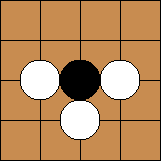
\includegraphics[width=\textwidth]{ex/Ex1-0.png}
\caption{Before Move}
\label{fig:ex1-0}
\end{subfigure}
\begin{subfigure}[b]{0.45\textwidth}
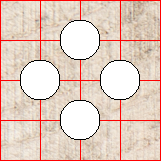
\includegraphics[width=\textwidth]{ex/Ex1-1.png}
\caption{After Move}
\label{fig:ex1-1}
\end{subfigure}
\caption{Example 1: The black stone is “captured” as the top white stone is placed because the black stone has no liberty left.}
\label{fig:ex1}
\end{figure}


\begin{figure}[!h]
\centering
\begin{subfigure}[b]{0.45\textwidth}
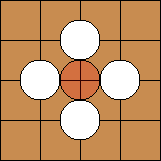
\includegraphics[width=\textwidth]{ex/Ex2-0.png}
\caption{Middle point is invalid}
\label{fig:ex2-0}
\end{subfigure}
\caption{Example 2: A black stone cannot be placed in the middle of the four white stones because this would lead to self-capture.}
\label{fig:ex2}
\end{figure}

\begin{figure}[!h]
\centering
\begin{subfigure}[b]{0.45\textwidth}
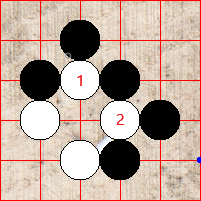
\includegraphics[width=\textwidth]{ex/Ex3-0.png}
\caption{Before Move}
\label{fig:ex3-0}
\end{subfigure}
\begin{subfigure}[b]{0.45\textwidth}
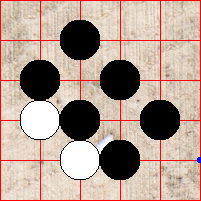
\includegraphics[width=\textwidth]{ex/Ex3-1.png}
\caption{After Move}
\label{fig:ex3-1}
\end{subfigure}
\caption{Example 3: A black stone can be placed in the middle of the four white stones because 1 and 2 will be immediately captured before the self-capture rule is applied. }
\label{fig:ex3}
\end{figure}


\begin{figure}[!h]
\centering
\begin{subfigure}[b]{0.45\textwidth}
\centering
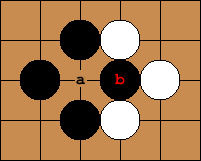
\includegraphics[width=\textwidth]{ex/Ex4-0.png}
\caption{Before Move}
\label{fig:ex4-0}
\end{subfigure}
\begin{subfigure}[b]{0.45\textwidth}
\centering
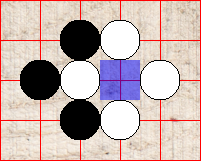
\includegraphics[width=\textwidth]{ex/Ex4-1.png}
\caption{After Move - Blue Square to represent KO}
\label{fig:ex4-1}
\end{subfigure}
\caption{Example 4: Once a white stone is placed at a to capture the black stone at b , black stone cannot be played at b next turn by the opponent to capture the white stone placed at a.}
\label{fig:ex4}
\end{figure}


\begin{figure}[!h]
\centering
\begin{subfigure}[b]{0.45\textwidth}
\centering
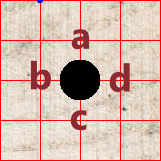
\includegraphics[width=0.666\textwidth]{ex/Ex5-0.png}
\caption{A black stone and its liberties}
\label{fig:ex5-0}
\end{subfigure}
\begin{subfigure}[b]{0.45\textwidth}
\centering
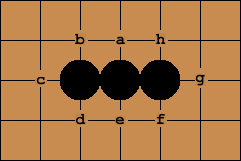
\includegraphics[width=\textwidth]{ex/Ex5-1.png}
\caption{A black stone string and its liberties}
\label{fig:ex5-1}
\end{subfigure}
\caption{Example 5: The liberties of a stone or a string of stone are the empty adjacent intersections.  In ~\autoref{fig:ex5-0} intersections a,b,c and d are the liberties of the black stone.
In ~\autoref{fig:ex5-1} intersections a to g are the liberties of the black stone string but h is not a liberty due to the white stone that occupies it.}
\label{fig:ex5}
\end{figure}

\begin{figure}[!h]
\centering
\begin{subfigure}[b]{0.45\textwidth}
\centering
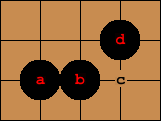
\includegraphics[width=\textwidth]{ex/Ex6-0.png}
\caption{Before Move}
\label{fig:ex6-0}
\end{subfigure}
\begin{subfigure}[b]{0.45\textwidth}
\centering
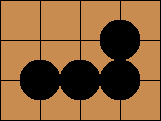
\includegraphics[width=\textwidth]{ex/Ex6-1.png}
\caption{After Move}
\label{fig:ex6-1}
\end{subfigure}
\caption{Example 6: The black stones a and b are connected but d is not connected to either a or b. If a black stone is placed at c then a,b,c and d are all said to be connected to each other.}
\label{fig:ex6}
\end{figure}


\section{Related Works}
Martin Müller's Explorer [2] was a strong program developed with the intention of playing Go. It captures key aspects of computer Go which can be used along with the minimax algorithm in one program. Explorer can evaluate the board in terms of safe territories for each player and can distinguish between safe stones and safe territories. Safe stones are any stones that are deemed alive but safe territories requires that no opponent stones can live within the safe stones. Explorer also takes into consideration of Semeai positions which are capturing races that occur within a game of Go. The victor of Semeai can be determined early sometimes and hence doing so during the evaluation could save searching further during minimax.

While explorer aims to play the Go, this project aims to create a program to solve life and death situations. To do so, determining safety of keystones within a problem is important.  Safety of strings during the board evaluation can determine whether a correct move is made or not.







\chapter{Requirements}


The project requires a well-defined and clear list of requirements due to the possible scale of it. Time constraints and resources available had to be taken to consideration before further work on the project was done. More precisely there was a need for identifying key aspects of the goals of this project and put them into more concrete requirements, so they can be implemented accordingly to achieve the goals of the project. Also, to keep track and have a streamlined work flow throughout the project the following requirements and scope were set.

\section{Functional Requirements}
To begin with the project's first milestone's aim which is to create an AI to play against user in Go life and death problems using brute force search. To achieve this, certain key requirements needed to be met:

The basic Go board should be displayed on the screen in which users can place stones in turn through mouse clicks. It needs comply to all the rules of Go and should capture and remove stones from the Board automatically after each turn. The program must be able to generate all the valid moves that can be made each turn and highlight them on the screen. Furthermore, the program itself must let the user create Go problems within it. To do so, split the program into two modes of use, an editor mode and player mode.

Editor mode needs to permit the user the ability to place black and white stones where needed without needing to take turns to create the initial board state they want their problems to be in. The state of the board needs to be valid always such that rules of Go would allow the board position to occur in normal play for it be able to be created in editor mode. Captured stones must be removed from the board and also only one ko point exists on the board. Editor should be able to define the boundary of play area, specifically to be able to choose which points on the board are in play for the problem. Keystones should be place able via editor mode, the keystone/s’s purpose is to identify the stone in which the problem revolves around. Users should also be able to select who to play first, and whether to capture or keep alive the keystone/s. Finally, the editor mode is required to let the user to create a text description of the problem and save the entire problem into a text file. The save files needs be human readable and the program should be able to load them back to either edit the problem or to play them.
The player mode is required allow the user to play through problems. This means it must allow users to load problems in from save files and play them out against the computer. To achieve the goal of creating an AI to play the game, there needs to be some features within the program to help with debugging. The ability to reset the problem back to original state, undo or redo a move and to also disable or enable the AI when required must be implemented into player mode.

The final requirement to achieve the first milestone needs to be addressed. There is a need for the program to contain a simple but effective Alpha-Beta pruning search algorithm to allow the correct move to be determined by the computer given board of stones and which colour’s turn it is, so that the computer can make that move to allow that colour to win. To make things simpler when problems are created, keystone/s needs to be placed on the board to allow the algorithm to surround its evaluations according to the status of the keystone/s on the board. For example, if the current turn is white and there is/are black keystone/s on board then the AI run the search algorithm and would evaluate to choose the move which would lead for the black keystone/s to be captured.

To achieve final aim of the project which is to adapt the AI created in the first part of the project to solve larger and more complex problems the following critical requirements are needed:

To introduce heuristics to the brute force Alpha-Beta search algorithm the program should contain a specialised module which evaluate the state of the board of each colour and returns how good or bad it is. This is so that given depth cut off to the search tree is implemented, the algorithm can return a value more accurately predict what would have been the result if the search has continued deeper. The AI must also use a complex move generator which given set of valid moves it picks certain number of moves and orders them according to the likelihood of being a good move using heuristics. Then the AI searches through this list of moves before going through and checking all the other possible valid moves.

In addition, with these critical requirements some sub-requirements are needed to help with testing and to finalise the product. A set of Go problems are needed to be created and built into the product. This is to allow users to immediately try out the player mode without needing to create problems by themselves, will be especially be useful for players new to Go. Another feature needed to be implemented was a valid move checker, to return a list of all possible moves either to enforce the rules of the game to the users to play properly or to allow the AI playing against the human to have a way to generate a list of possible moves to search through.


With all the requirements of the project it had become evident the scope of the project could vary drastically. To create a perfect Go playing AI on full 19x19 board would be far from achievable given the time and resources put into the project. The main constraints to decide the scope were:
\begin{itemize}
	\item Time given for AI to search and find the correct move?
	\item The number of given valid moves a problem contains which the AI should solve?
\end{itemize}
These two constraints are closely related to each other, more valid moves the AI is expected to handle the more time it should be allowed but with an upper bound set to allow users to interact and solve the problems without waiting too long. These were needed to be adjustable according to the feedback given by user testing. Hence the AI had to be built in way to allow for flexibility regarding these two parameters. To do so, the program gives the ability to choose what depth the AB pruning algorithm searches to before it cuts off to the user. This directly affect both run time of the algorithm and scale of the problem as bigger problems can be allowed with smaller cut off depth also would lead to less time required.


\section{Non-Functional Requirements}
Throughout the project some non-functional requirements where discovered and needed to be addressed , following categories were made to specify the different criteria GoLD need to achieve.

Performance / Time - Important concern was the time factor a user wants to spend during the process of solving problems using GoLD.

Usability - Another concern was the ease of use , whether the program is simple and understandable for untrained users.

Reliability – The program should be able to cope with any kind of user inputs and should maintain running with any failures or crashes.



\chapter{Design}


\section{Brute Force Search}
For the computer to play against a human it needs to be able to determine the best move it can make. Simplest way to do this is by searching through the game tree and determining the end results of each valid move. The game tree consists of every single board position that is possible to occur from the current board position. Board position refers to the state of the entire board, each sub tree of the game tree is the result of making a valid move in the current board position. Every sub tree is explored deeper until the resulting board position is in a game ending state. This type of search can be referred to as a brute force search and within GoLD the ability to “brute force search” is essential as it is the foundation to which rest of the program’s AI is built upon.

\subsection{Alpha-Beta Pruning Search Algorithm}

The basis of finding the correct move within GoLD is the Alpha-Beta pruning search algorithm. Alpha-Beta is an algorithm which optimises the simple minimax algorithm and returns the same results in less time. Minimax is perfect for searching Go’s game tree where two players are playing, and one player’s gains are directly linked to the other player’s losses. A simple implementation of minimax will search each valid move of the initial board position and choose a move which results in victory even if the opponent plays perfectly, if there is such a move. In terms of Go given the computer is black, during the search minimax alternates between playing as black and white until an end goal is reached and then chooses an initial move which leads black to win.

Within life and death situation of this project the end goal is easy to determine if the attacking player as no valid moves and the keystones remain on the board then the defending player has won. Alternatively, as soon as all the keystones on the board is captured then the attacking player has won. In a real game of Go, results of end games are not so simple. There might be multiple solutions which results in capture of all the keystones’ string but there might only be one solution which will do so without allowing for losses on other parts of the board for the attacking player. This is ignored with GoLD as we are only interested in the result of life and death problems not the outcome of the board. Hence any solution which captures the given keystones are sufficient for the project. An example of minimax algorithm used in a simple number game is show in ~\autoref{fig:MinMaxNumTree}

\begin{figure}[!h]
\centering
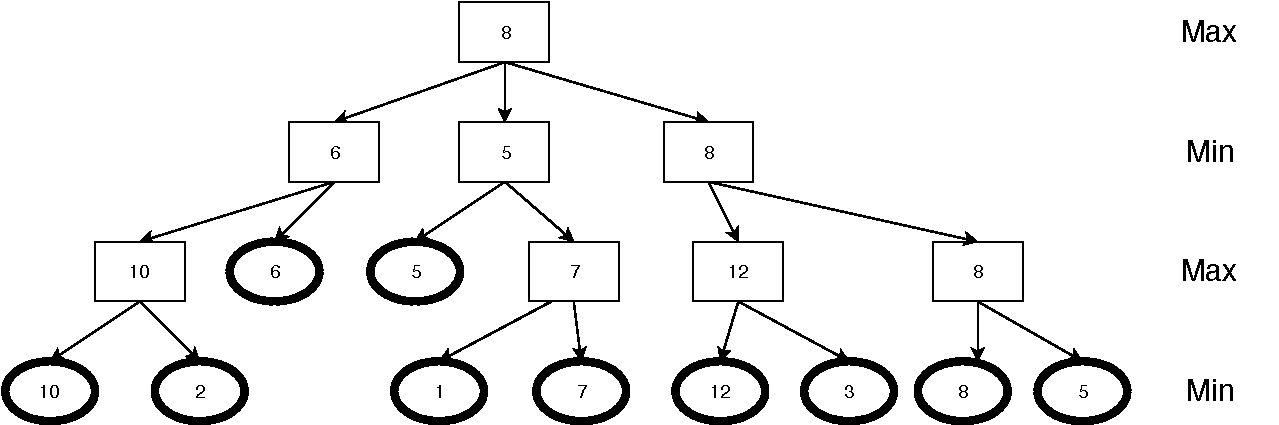
\includegraphics[width=0.9\textwidth]{MinMaxNumTree}
\caption{Minimax being used for simple number game. Best score the maximizing player can get is 8. Even though scoring 10 and 12 are possible when minimizing player plays optimally the score can’t out be achieved.}
\label{fig:MinMaxNumTree}
\end{figure}

The alpha-beta pruning algorithm is smart improvement to reduce the search time of the minimax algorithm. It allows for the correct result to be determined without having to search through every possible sub tree of the initial game tree. It uses alpha and beta values to determine whether further search is required or not. To begin with alpha is set -inf and beta is set to +inf, these values are passed down through the layers of the search algorithm and changes to the alpha or beta values only affect the deeper layers of the search. If a maximizing layer finds a move which gives a score greater than the previous best move of that layer, then the alpha value of that layer is increased to the value of new best move. If a minimizing layer finds a move which gives a score less than the previous best move of that layer, then the beta value of that layer is decreased to the value of new best move.  After each move is searched in a layer, the algorithm checks if the alpha value is greater than or equal to the beta value and if it is the algorithm decides that checking more moves in that layer is pointless and returns the best move back to previous layer. This results drastic improvements to the minimax algorithm without changing the result as it cuts out the search of many branches of the game tree which doesn’t affect the result of the algorithm. An example of Alpha-Beta pruning algorithm used for the same simple number game is show in ~\autoref{fig:ABNumTree}


\begin{figure}[!h]
\centering
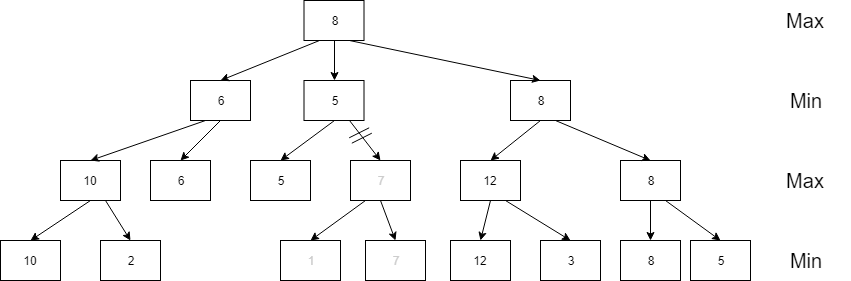
\includegraphics[width=0.9\textwidth]{ABNumTree}
\caption{Same simple number game using alpha-beta pruning. In the second layer of the second sub three after searching the first child node which returns 5 the algorithm cuts off from any further search in that sub tree as it realises the first sub tree will always be better than 5. }
\label{fig:ABNumTree}
\end{figure}

Pseudocode of the implementation of alpha-beta algorithm for the program is as follows:







\subsection{Suicidal Move Removal}
Keystones are an absolute objective in the program, they are one of the reference points which the program checks to see if the problem is solved or not. From the defender’s perspective any moves that are detrimental to the immediate safety of keystones need to be removed from the list of valid moves to be searched by alpha-beta algorithm. This entails removing any suicidal moves that decreases the number of liberties of a keystring to 1.

A solution can be derived from the fact that placing 1 stone can at maximum only remove 1 liberty of a keystring. Hence, GoLD only needs to look at the moves that places a stone in liberties of keystrings with 2 liberties, anymore liberties would ensure at least 2 liberties would remain intact if a stone was to be placed on a liberty. For keystrings with 2 liberties, placing in one of those 2 liberties does not automatically mean it is a suicidal move for two reasons: Move captures an opponent string; Move would increase or maintain the liberty count. If any of these two reasons are met, then the move is not suicidal.

\begin{itemize}
	\item Both liberties of the keystring is added to the suicidal move list.
	\item Moves that places a stone in the liberty of any opponent string which is in Atari is removed from the suicidal move list.
    \item Moves that connects the keystring to another string which fits the following criteria are removed from the suicidal move list: Must be same colour as the keystring; Has more than 2 liberties or has 2 liberties which are not the same 2 liberties of the keystring.
    \item Moves that places a stone adjacent to any empty point which is not a liberty of the keystring are removed from the suicidal move list.
\end{itemize}

After these checks are done for all the keystrings, any moves remaining in the suicidal moves list are removed from the valid moves list – this new list of moves is referred to as the good moves list. The good moves list is used during AB search instead of valid moves list to save time by not searching valid moves which would lead to immediate capture of keystones. If no moves are considered “good” then the defending player is to pass instead of making a bad move during AB search


\section{Heuristics}

The Alpha-Beta pruning search algorithm by itself is great improvement over the standard minimax but with this improvement the sheer size of the search space can become quickly overwhelming for it to handle in reasonable time. Alpha-Beta even at best case has complexity of O($\sqrt{b^d}$) and at worst O($b^d$) which means for problems with greater area of search space or problems that require search into further depths to come to a terminating state could incalculable amount of time. For this reason, we have to introduce heuristics within the Alpha-Beta search to allow the search to come with a quicker solution rather than the perfect solution. There are quite a few methods of implementing heuristics within the Alpha-Beta search, GoLD will be able to use few of these in combination or by themselves to restrict the time taken for the computer to respond to the user.

\subsection{Depth Limited Search with Board Evaluation}
Alpha-Beta search which will search deeper with no depth restriction until a terminal state is found are impractical. Best way to deal with this is to introduce a depth limit where once depth X is reached the search is not continued. Of course, the problem with this is that when cut offs occur the game state will not be in a terminal state and hence the alpha search needs to do some type of evaluation in order to return a score which is between the two opposing terminal state of being dead or alive. The alpha-beta search will have to evaluate the board position when the cut off depth is reached and return value which represents how good the board is for players. For example, if the board position will lead the attacking player to capture all the keystones then the board evaluation should return -5000  on the other hand if the board position is in favour of the defending team then it should return 5000. Creating a function which evaluates the board accurately is a difficult task and doing so which can perform at the level of humans is even more difficult. An important factor to consider when designing an evaluation function is also the time it takes evaluate a board position. More complex the evaluation function becomes the longer it takes to evaluate single a  board position hence the more time it takes to evaluate the board position every time the depth limit is reached.


\subsubsection{Pattern Matching Evaluation}

When evaluating a board position GoLD looks at the board similar to how humans would look at a board it tries to identify general patterns on the board to give values depending on pattern it finds. These patterns are based of the idea of eyes and eyes space. Identifying patterns which will lead to multiple eyes will be evaluated to very high score and hence the search will be able to recognise the group of stone will be able to live without further searching. General principle behind the patterns used in GoLD is to identify the number of eyes it can produce when fully played out and values according to this factor is added to the overall board score.

Most of the patterns used within GoLD have a distinct feature which is common in life and death problems which is that depending on who plays first the pattern/shape becomes dead or alive. Another words these shaped are unsettled and hence contains a vital point which will determine the number of eyes that can be produced by the shape. Figure 1a shows a pattern used in GoLD, the shape referred as straight three but with its corner stones. The vital point of this pattern is a , if white is able to play at a then the pattern is almost ensured to create two eyes unless white makes a mistake filling in the corners. The corners b, c, d and e are also important for this pattern if black is able to have stones in both b and c  or in d and e then the wall of shape becomes weak and hence the shape can become captured. Due to alternating play if white plays first in this situation then it will be played out as shown in Figure 1b where white is able to produce two real eyes.



\subsection{Pattern Searching}


\subsection{Move Generator}



\section{Overall Architecture}




\chapter{Implementation}

\section{Play Mode}

\section{Edit Mode}

\section{Game Board}

\section{Problem File}

\section{Pattern Searcher}








\chapter{Evaluation}

\section{Unit Testing}

\section{Evaluation of Heuristics}
\subsection{Types of Problems}
\subsection{Success Rate}

\section{Beta Testing with Go Players}
\subsection{Questionnaires}
\subsection{Interviews}






\chapter{Conclusion}

\section{Summary}

\section{Future Works}

\section{Reflection}


\chapter{References}
1.http://www.cs.cmu.edu/~wjh/go/rules/Japanese.html
2.Müller, M. (2002). POSITION EVALUATION IN COMPUTER GO. ICGA Journal, 25(4), pp.219-228.
3.Chikun, C. (1993). All About Life & Death. Ishi Pr.
4.Davies, J. (1996). Life and Death. Ishi Pr.
5.Cornelis Diederik van der Werf, E. (2004). AI techniques for the game of Go. [Maastricht]: UPM, Universitaire Pers Maastricht.
6.Akl, S.G., & Newborn, M. (1977). The principal continuation and the killer heuristic. ACM Annual Conference.
7.Huberman, B.J. (1968). A PROGRAM TO PLAY CHESS END GAMES.








\end{document}
